\documentclass[aspectratio=169]{beamer}
\usetheme{default}\usecolortheme{seahorse}
\setbeamertemplate{navigation symbols}{}
\setbeamertemplate{footline}[frame number]
\usepackage{graphicx}\usepackage{booktabs}
\setbeamertemplate{section in toc}{\inserttocsectionnumber.~\inserttocsection}
\title{What Cross-Modal Connectome Prediction Does and Does Not Buy}
\subtitle{Reconstruction, baselines, and downstream utility (Glasser; 4S456 in backup)}
\author{Adel Sahuc}\date{}
\begin{document}
\frame{\titlepage}
\section{Asymmetry}
\begin{frame}{1 · Cross-modal prediction is directional\,{\footnotesize[PCA$\rightarrow$PLS]}}\vfill\centering\large
\begin{tabular}{@{}lc@{}}\toprule \textbf{direction} & \textbf{demeaned r} \\\midrule FC$\rightarrow$SC & 0.136 \\ SC$\rightarrow$FC & 0.084 \\\midrule \textbf{ratio} & \textbf{1.61$\times$} \\\bottomrule\end{tabular}\vfill\end{frame}
\begin{frame}{1 · Cross-modal prediction is directional\,{\footnotesize[PCA$\rightarrow$PLS]}}\centering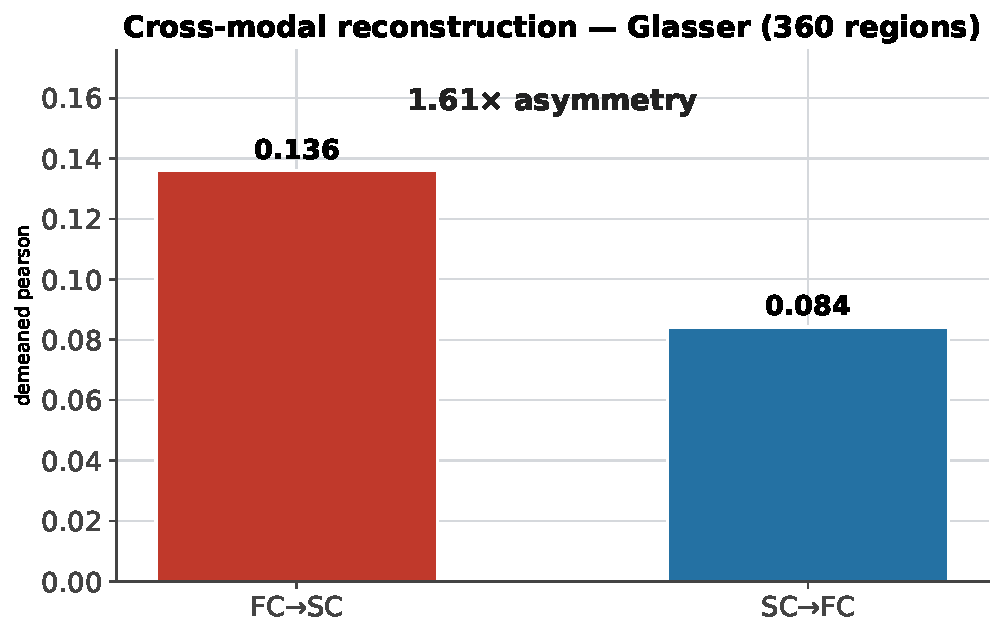
\includegraphics[height=0.66\textheight,width=\linewidth,keepaspectratio]{figures/simplified/asym_Glasser.pdf}\\[3pt]\begin{minipage}{0.95\linewidth}\scriptsize Across all three models the FC$\rightarrow$SC bars are $\sim$1.6$\times$ taller than SC$\rightarrow$FC: FC reconstructs SC's individual deviations far better than the reverse, and the ratio barely changes by model, so it is not an estimator artifact. Whisker = 25th--75th percentile across the 10 seeds; white circle = mean.\end{minipage}\end{frame}
\begin{frame}{2 · A cheap baseline beats cross-modal reconstruction\,{\footnotesize[PCA$\rightarrow$PLS]}}\vfill\centering\large
\begin{tabular}{@{}lcc@{}}\toprule \textbf{source} & \textbf{$\rightarrow$ SC} & \textbf{$\rightarrow$ FC} \\\midrule cross-modal connectome & 0.136 & 0.084 \\ brain volume (bv) & 0.162 & 0.049 \\ demographics (demo) & 0.130 & 0.111 \\ bv+demo & 0.169 & 0.100 \\ \textbf{connectome + bv+demo} & \textbf{0.171} & \textbf{0.105} \\ \bottomrule\end{tabular}\vfill\end{frame}
\begin{frame}{2 · A cheap baseline beats cross-modal reconstruction\,{\footnotesize[PCA$\rightarrow$PLS]}}\centering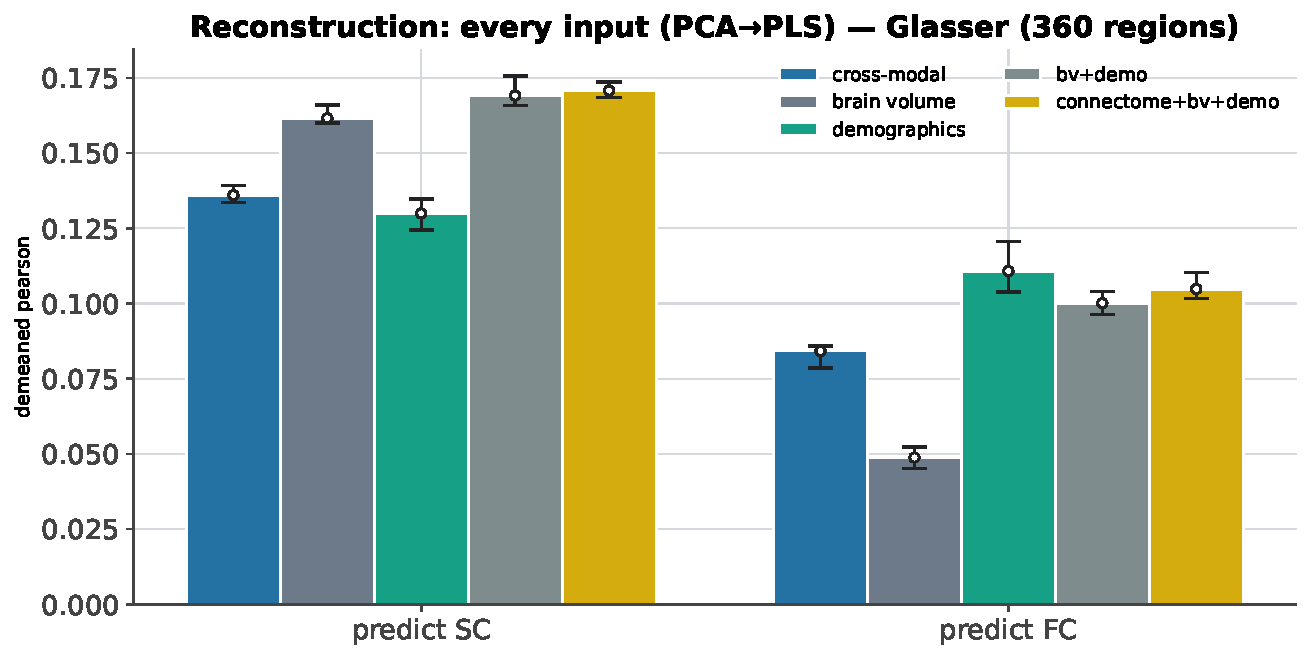
\includegraphics[height=0.66\textheight,width=\linewidth,keepaspectratio]{figures/simplified/baseline_Glasser.pdf}\\[3pt]\begin{minipage}{0.95\linewidth}\scriptsize For \emph{both} targets bv+demo matches or beats the cross-modal connectome: a cheap age+sex+volume vector reconstructs the missing connectome as well as the other modality does. Adding the connectome on top of bv+demo (gold) gives only a marginal extra, so the connectome adds little beyond subject information. Note the dissociation: bv (volume) wins for SC, demo wins for FC.\end{minipage}\end{frame}
\begin{frame}{3a · Predicting SC: every metric\,{\footnotesize[PCA$\rightarrow$PLS]}}\vfill\centering\small
\begin{tabular}{@{}lcccccc@{}}\toprule \textbf{input} & \textbf{demeaned r} & \textbf{raw r} & \textbf{top1} & \textbf{avg rank} & \textbf{mse} & \textbf{r$^2$} \\\midrule FC$\rightarrow$SC & 0.136 & 0.913 & 0.120 & 0.875 & 0.006 & -0.021 \\ bv$\rightarrow$SC & 0.162 & 0.915 & 0.086 & 0.864 & 0.005 & 0.014 \\ demo$\rightarrow$SC & 0.130 & 0.915 & 0.023 & 0.754 & 0.005 & 0.001 \\ bv+demo$\rightarrow$SC & 0.169 & 0.914 & 0.129 & 0.875 & 0.005 & 0.008 \\ \textbf{FC+bv+demo$\rightarrow$SC} & \textbf{0.171} & \textbf{0.913} & \textbf{0.169} & \textbf{0.914} & \textbf{0.005} & \textbf{-0.009} \\ \bottomrule\end{tabular}\vfill\end{frame}
\begin{frame}{3a · Predicting SC: comparable metrics\,{\footnotesize[PCA$\rightarrow$PLS]}}\centering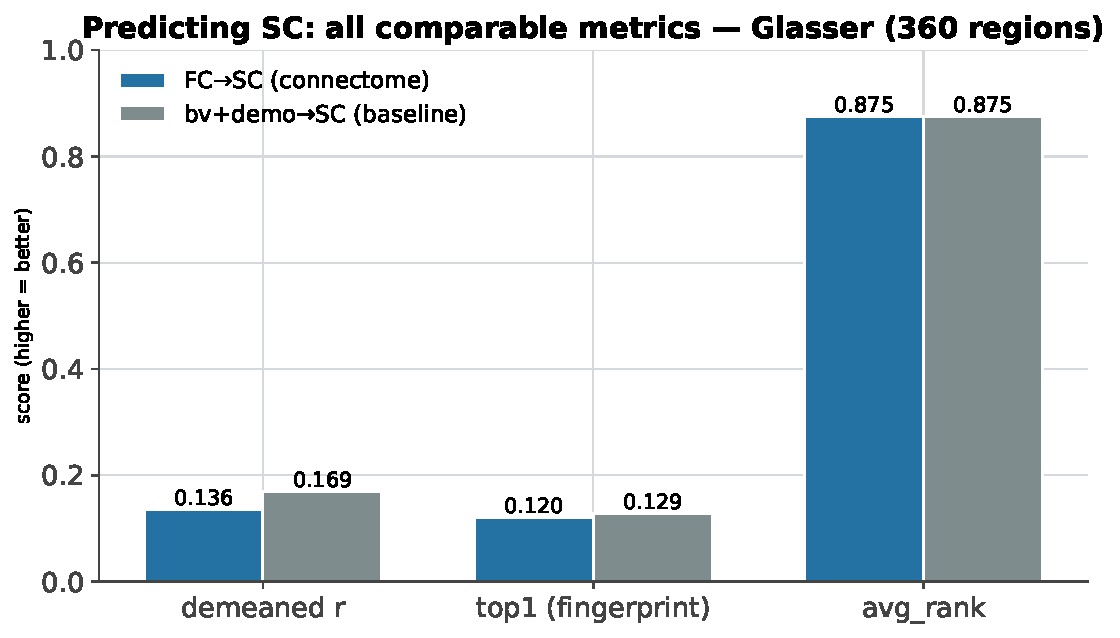
\includegraphics[height=0.66\textheight,width=\linewidth,keepaspectratio]{figures/simplified/metrics_SC_Glasser.pdf}\\[3pt]\begin{minipage}{0.95\linewidth}\scriptsize Raw r is $\sim$0.9 for every input (dominated by the shared group-mean connectome, so uninformative); demeaned r is the honest individual-deviation metric, where bv+demo leads. Whisker = 25th--75th percentile over the 10 seeds.\end{minipage}\end{frame}
\begin{frame}{3b · Predicting FC: every metric\,{\footnotesize[PCA$\rightarrow$PLS]}}\vfill\centering\small
\begin{tabular}{@{}lcccccc@{}}\toprule \textbf{input} & \textbf{demeaned r} & \textbf{raw r} & \textbf{top1} & \textbf{avg rank} & \textbf{mse} & \textbf{r$^2$} \\\midrule SC$\rightarrow$FC & 0.084 & 0.828 & 0.049 & 0.714 & 0.014 & -0.056 \\ bv$\rightarrow$FC & 0.049 & 0.833 & 0.012 & 0.623 & 0.014 & -0.022 \\ demo$\rightarrow$FC & 0.111 & 0.837 & 0.013 & 0.671 & 0.014 & -0.002 \\ bv+demo$\rightarrow$FC & 0.100 & 0.834 & 0.024 & 0.685 & 0.014 & -0.019 \\ \textbf{SC+bv+demo$\rightarrow$FC} & \textbf{0.105} & \textbf{0.829} & \textbf{0.054} & \textbf{0.743} & \textbf{0.014} & \textbf{-0.047} \\ \bottomrule\end{tabular}\vfill\end{frame}
\begin{frame}{3b · Predicting FC: comparable metrics\,{\footnotesize[PCA$\rightarrow$PLS]}}\centering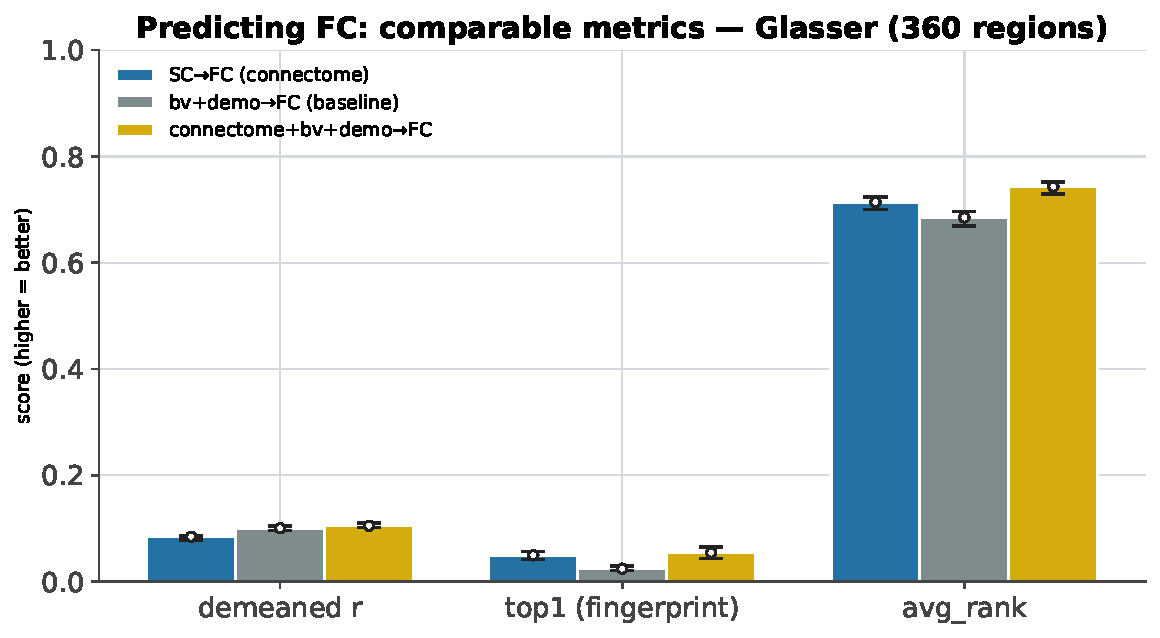
\includegraphics[height=0.66\textheight,width=\linewidth,keepaspectratio]{figures/simplified/metrics_FC_Glasser.pdf}\\[3pt]\begin{minipage}{0.95\linewidth}\scriptsize Same picture predicting FC, with one twist: the real connectome (SC) beats bv+demo on the fingerprint metrics (top1, avg rank), i.e.\ it carries subject-identity information the cheap baseline lacks.\end{minipage}\end{frame}
\begin{frame}{4 · Downstream cognition: only observed FC helps\,{\footnotesize[BayesianRidge]}}\vfill\centering\footnotesize
\begin{tabular}{@{}lcccc@{}}\toprule \textbf{input} & \textbf{CogCryst r} & \textbf{Total lift} & \textbf{Fluid lift} & \textbf{Cryst lift} \\\midrule bv+demo (baseline) & 0.354 & +0.000 & +0.000 & +0.000 \\ \textbf{observed FC} & \textbf{0.487} & \textbf{+0.088} & \textbf{+0.044} & \textbf{+0.133} \\ observed SC & 0.253 & -0.111 & -0.120 & -0.101 \\ observed FC + SC & 0.490 & +0.090 & +0.048 & +0.136 \\ \textbf{observed FC + bv+demo} & \textbf{0.516} & \textbf{+0.115} & \textbf{+0.073} & \textbf{+0.162} \\ observed SC + bv+demo & 0.319 & -0.050 & -0.066 & -0.035 \\ predicted SC & 0.344 & -0.018 & -0.053 & -0.010 \\ predicted FC & 0.219 & -0.113 & -0.097 & -0.135 \\ predicted SC + bv+demo & 0.415 & +0.040 & +0.022 & +0.061 \\ predicted FC + bv+demo & 0.314 & -0.038 & -0.038 & -0.040 \\ \bottomrule\end{tabular}\vfill\end{frame}
\begin{frame}{4 · Downstream cognition: only observed FC helps\,{\footnotesize[BayesianRidge]}}\centering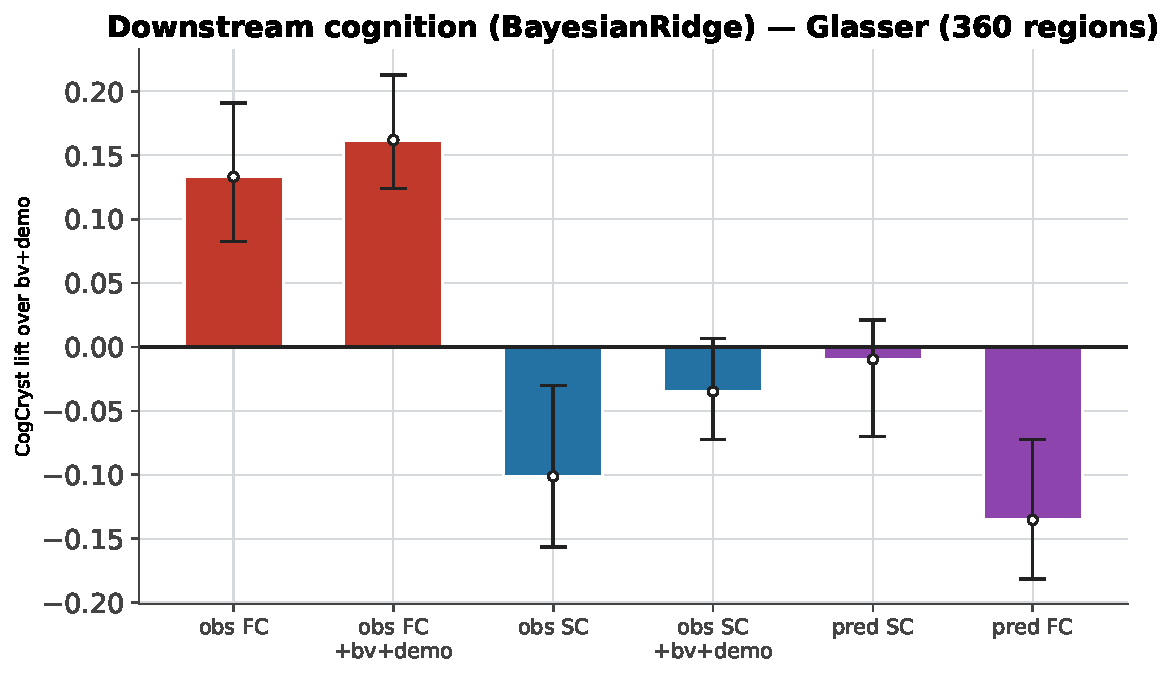
\includegraphics[height=0.66\textheight,width=\linewidth,keepaspectratio]{figures/simplified/cog_Glasser.pdf}\\[3pt]\begin{minipage}{0.95\linewidth}\scriptsize Only observed FC and observed FC+bv+demo rise above zero (beat the baseline). Observed SC and both predicted connectomes sit at or below zero; predicted FC is actively harmful. Wide whiskers (25--75th pct over seeds) show even the FC lift is variable.\end{minipage}\end{frame}
\begin{frame}{5 · Downstream family: the predicted connectome carries it\,{\footnotesize[PCA$\rightarrow$PLS]}}\vfill\centering\small
\begin{tabular}{@{}lccc@{}}\toprule \textbf{predictor} & \textbf{MZ} & \textbf{DZ} & \textbf{sibling} \\\midrule observed SC & 0.999 & 0.938 & 0.863 \\ observed FC & 0.990 & 0.886 & 0.823 \\ predicted SC (raw) & 0.974 & 0.798 & 0.680 \\ \textbf{predicted SC (demog removed)} & \textbf{0.989} & \textbf{0.823} & \textbf{0.810} \\ predicted FC (raw) & 0.910 & 0.756 & 0.710 \\ predicted FC (demog removed) & 0.918 & 0.741 & 0.743 \\ \textbf{combined predicted SC} & \textbf{0.897} & \textbf{0.701} & \textbf{0.505} \\ bv+demo baseline & 0.951 & 0.800 & 0.563 \\ \bottomrule\end{tabular}\vfill\end{frame}
\begin{frame}{5 · Downstream family: the predicted connectome carries it\,{\footnotesize[PCA$\rightarrow$PLS]}}\centering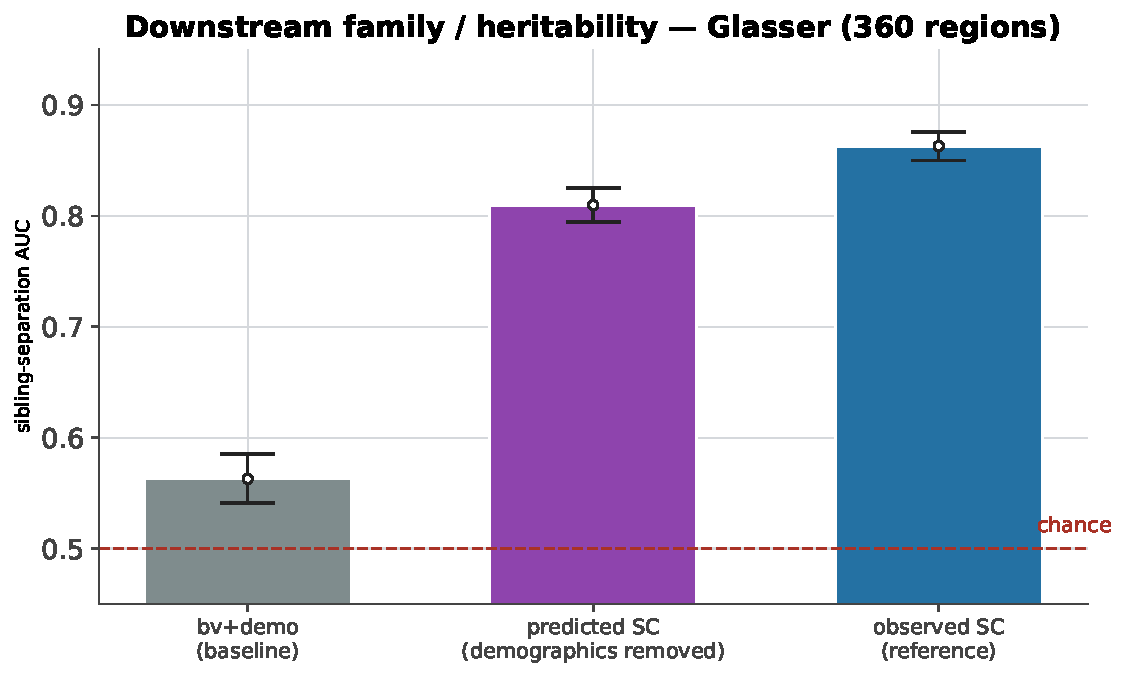
\includegraphics[height=0.66\textheight,width=\linewidth,keepaspectratio]{figures/simplified/family_Glasser.pdf}\\[3pt]\begin{minipage}{0.95\linewidth}\scriptsize Predicted SC separates siblings far above the bv+demo baseline and close to observed SC: the predicted connectome keeps heritable family structure. Whisker = bootstrap 95\% CI (family is a single pipeline with no seed split).\end{minipage}\end{frame}
\begin{frame}{6 · Are the results model-dependent?}\vfill\centering\footnotesize Headlines replicate across models; the only divergences are PLS's low oracle and KernelRidge's unstable scalar rows.\\[6pt]\begin{tabular}{@{}lccc@{}}\toprule \textbf{reconstruction} & \textbf{PCA$\rightarrow$PLS} & \textbf{BayesianRidge} & \textbf{KernelRidge} \\\midrule FC$\rightarrow$SC & 0.136 & 0.166 & 0.133 \\ SC$\rightarrow$FC & 0.084 & 0.104 & 0.081 \\ \textbf{asymmetry ratio} & \textbf{1.61$\times$} & \textbf{1.60$\times$} & \textbf{1.65$\times$} \\ SC$\rightarrow$SC oracle & 0.376 & 0.648 & 0.648 \\ \bottomrule\end{tabular}\\[8pt]\begin{tabular}{@{}lccc@{}}\toprule \textbf{CogCryst lift} & \textbf{PCA$\rightarrow$PLS} & \textbf{BayesianRidge} & \textbf{KernelRidge} \\\midrule obs FC & +0.095 & +0.133 & +0.181 \\ obs SC & -0.009 & -0.101 & +0.088 \\ pred FC & -0.097 & -0.135 & +0.019 \\ \bottomrule\end{tabular}\vfill\end{frame}
\begin{frame}{6 · Are the results model-dependent?}\centering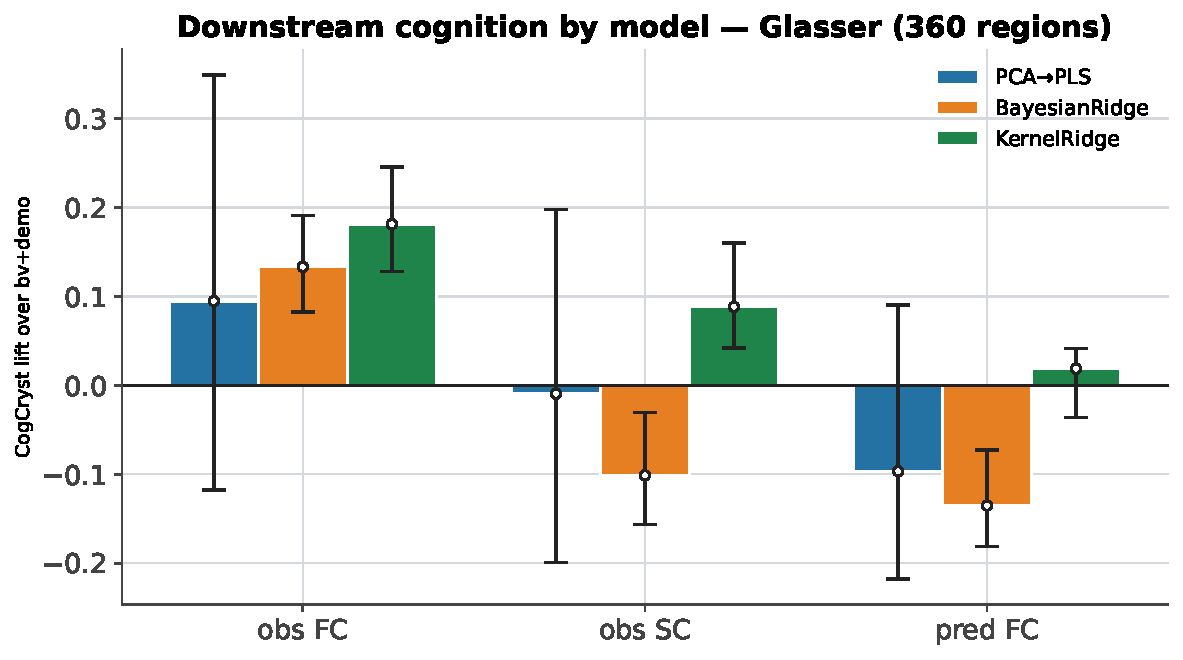
\includegraphics[height=0.66\textheight,width=\linewidth,keepaspectratio]{figures/simplified/models_Glasser.pdf}\\[3pt]\begin{minipage}{0.95\linewidth}\scriptsize The observed-FC cognition lift is positive under all three models, but the negatives (obs SC, pred FC) flip sign under KernelRidge (green): KernelRidge's scalar regression is numerically unstable, which is why cognition is reported with BayesianRidge.\end{minipage}\end{frame}
\section{Takeaways}\begin{frame}{Takeaways}\large\begin{enumerate}\item Cross-modal prediction is \textbf{real and directional}: FC$\rightarrow$SC $>$ SC$\rightarrow$FC (1.61$\times$).\item But a \textbf{cheap bv+demo baseline beats it} at reconstruction --- only the \emph{fingerprint/identity} signal is uniquely connectomic.\item Downstream, signal splits cleanly: \textbf{observed FC} carries (crystallized) cognition; \textbf{predicted SC} carries family/heritable signal.\end{enumerate}\end{frame}
\begin{frame}\centering\vfill{\Huge Thank you}\\[8pt]\large Questions?\\[12pt]\normalsize Backup: deeper dives (Q1, Q2), then 4S456 replication.\vfill\end{frame}
\section{Backup: deeper dives (Glasser)}
\begin{frame}{Q1 · Can a predicted connectome beat the real one?\,{\footnotesize[BayesianRidge]}}\vfill\centering\footnotesize Predicted SC beats \emph{observed} SC for cognition --- because predicted SC is a projection of FC (the strong modality). It still loses to FC itself.\\[6pt]\begin{tabular}{@{}lcc@{}}\toprule \textbf{input} & \textbf{Glasser} & \textbf{4S456} \\\midrule observed SC & -0.101 & -0.095 \\ predicted SC & -0.010 & -0.012 \\ observed SC + bv+demo & -0.035 & -0.042 \\ \textbf{predicted SC + bv+demo} & \textbf{+0.061} & \textbf{+0.056} \\ \midrule \textit{(source) observed FC + bv+demo} & \textit{+0.162} & \textit{+0.146} \\ \bottomrule\end{tabular}\\[8pt]\footnotesize …but the flip is estimator-specific:\\[3pt]\begin{tabular}{@{}lccc@{}}\toprule \textbf{CogCryst lift (Glasser)} & \textbf{PCA$\rightarrow$PLS} & \textbf{BayesianRidge} & \textbf{KernelRidge} \\\midrule predicted SC + bv+demo & +0.019 & +0.061 & +0.017 \\ observed SC + bv+demo & +0.050 & -0.035 & +0.128 \\ \midrule predicted $>$ observed? & no & \textbf{yes} & no \\ \bottomrule\end{tabular}\vfill\end{frame}
\begin{frame}{Q1 · Predicted SC beats observed SC --- but never the source\,{\footnotesize[BayesianRidge]}}\centering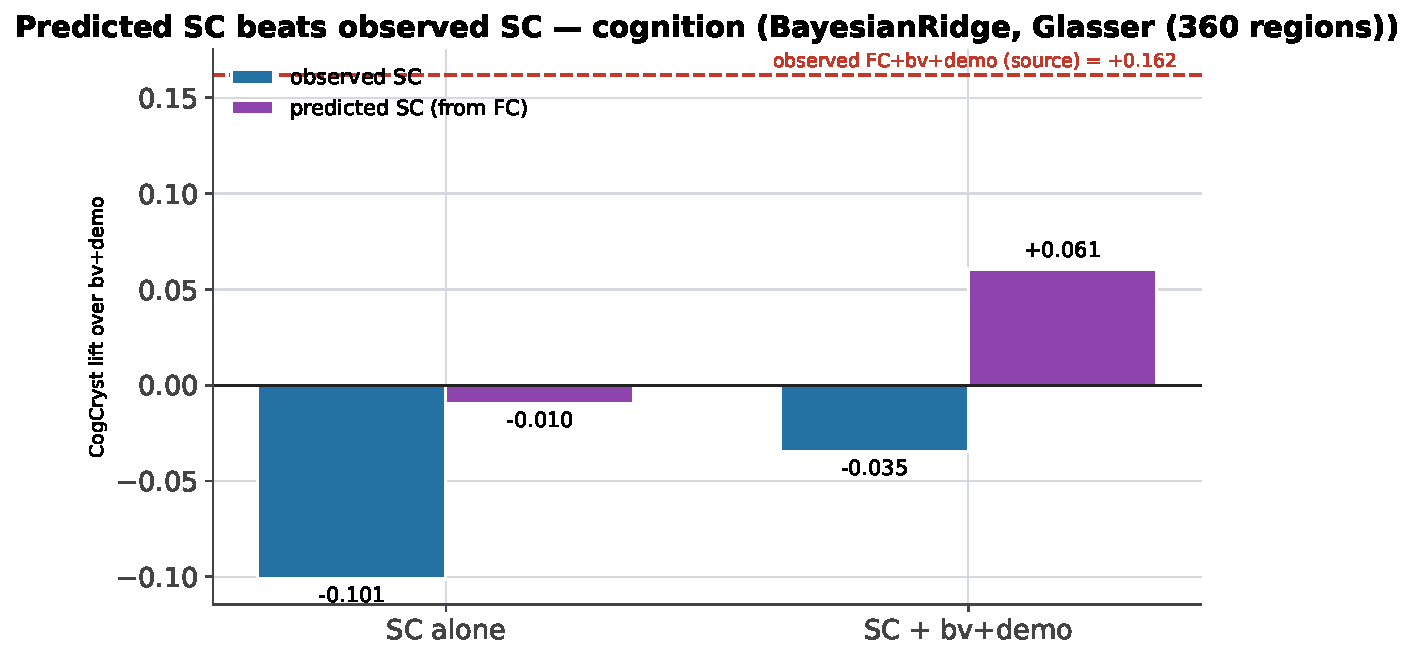
\includegraphics[height=0.66\textheight,width=\linewidth,keepaspectratio]{figures/simplified/q1_Glasser.pdf}\\[3pt]\begin{minipage}{0.95\linewidth}\scriptsize Predicted SC (purple) beats observed SC (blue) because predicted SC is a projection of FC, the modality that carries cognition. It never reaches observed FC itself (dashed line): you would always do better using FC directly.\end{minipage}\end{frame}
\begin{frame}{Q2 · Family signal across relatedness (MZ / DZ / sibling)\,{\footnotesize[PCA$\rightarrow$PLS]}}\vfill\centering\footnotesize A genetic dose-response; the reconstruction-optimized \emph{combined} predictor collapses to chance for siblings.\\[6pt]\begin{tabular}{@{}lccc@{}}\toprule \textbf{predictor} & \textbf{MZ twins} & \textbf{DZ twins} & \textbf{siblings} \\\midrule observed SC & 0.999 & 0.938 & 0.863 \\ predicted SC & 0.989 & 0.823 & 0.810 \\ predicted FC & 0.918 & 0.741 & 0.743 \\ combined predicted SC & 0.897 & 0.701 & 0.505 \\ bv+demo baseline & 0.951 & 0.800 & 0.563 \\ \bottomrule\end{tabular}\vfill\end{frame}
\begin{frame}{Q2 · Heritability gradient \& the objective tradeoff\,{\footnotesize[PCA$\rightarrow$PLS]}}\centering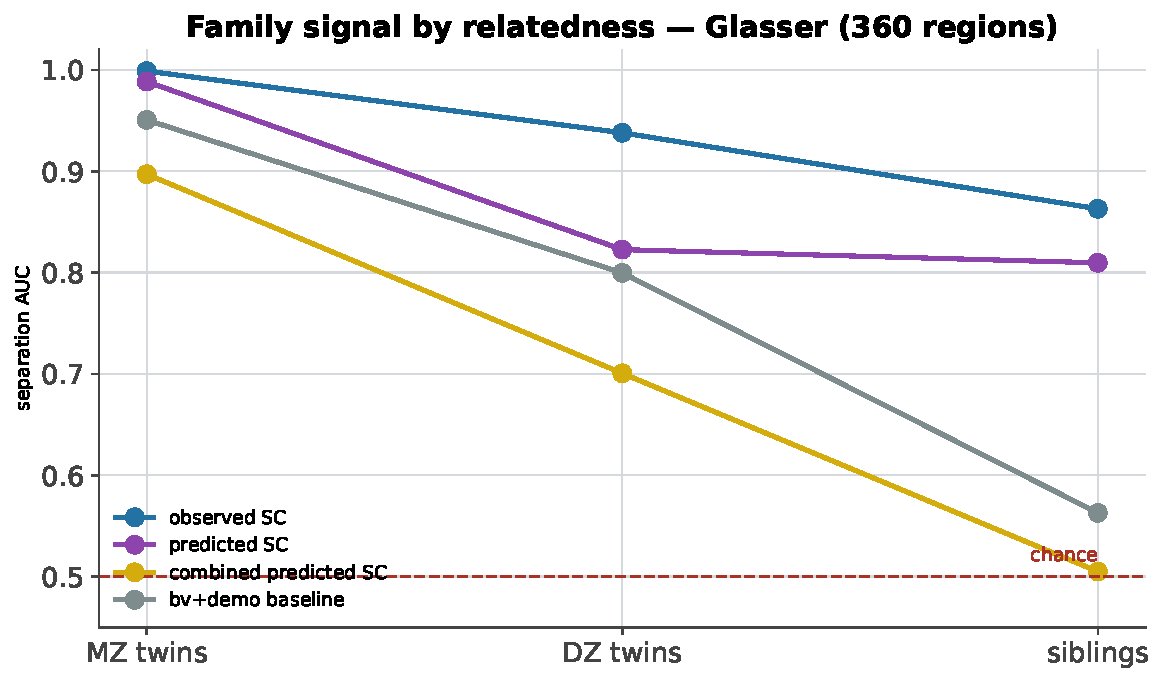
\includegraphics[height=0.66\textheight,width=\linewidth,keepaspectratio]{figures/simplified/q2_Glasser.pdf}\\[3pt]\begin{minipage}{0.95\linewidth}\scriptsize Every predictor weakens from MZ twins to DZ twins to siblings (a genetic dose-response). The combined predictor (gold) falls to the chance line at siblings: optimizing for reconstruction discards the fine-grained family signal.\end{minipage}\end{frame}
\begin{frame}{Q3 · Can a prediction beat the connectome it came from?\,{\footnotesize[BayesianRidge]}}\vfill\centering\footnotesize Predicted FC beats its source SC on the noisy targets (a denoising effect) --- but both stay below the baseline; predicted SC never beats its source FC.\\[8pt]\begin{tabular}{@{}lccc@{}}\toprule \textbf{input (CogXxx pearson r)} & \textbf{CogTotal} & \textbf{CogFluid} & \textbf{CogCryst} \\\midrule bv+demo (baseline) & 0.359 & 0.283 & 0.354 \\ \midrule observed FC & 0.447 & 0.327 & 0.487 \\ $\rightarrow$ predicted SC & 0.341 & 0.230 & 0.344 \\ observed FC + bv+demo & 0.474 & 0.356 & 0.516 \\ $\rightarrow$ predicted SC + bv+demo & 0.399 & 0.305 & 0.415 \\ \midrule observed SC & 0.248 & 0.163 & 0.253 \\ $\rightarrow$ predicted FC & 0.247 & \textbf{0.186} & 0.219 \\ observed SC + bv+demo & 0.309 & 0.217 & 0.319 \\ $\rightarrow$ predicted FC + bv+demo & \textbf{0.321} & \textbf{0.245} & 0.314 \\ \bottomrule\end{tabular}\vfill\end{frame}
\begin{frame}{Q3 · Prediction beats source only as `less harmful'\,{\footnotesize[BayesianRidge]}}\centering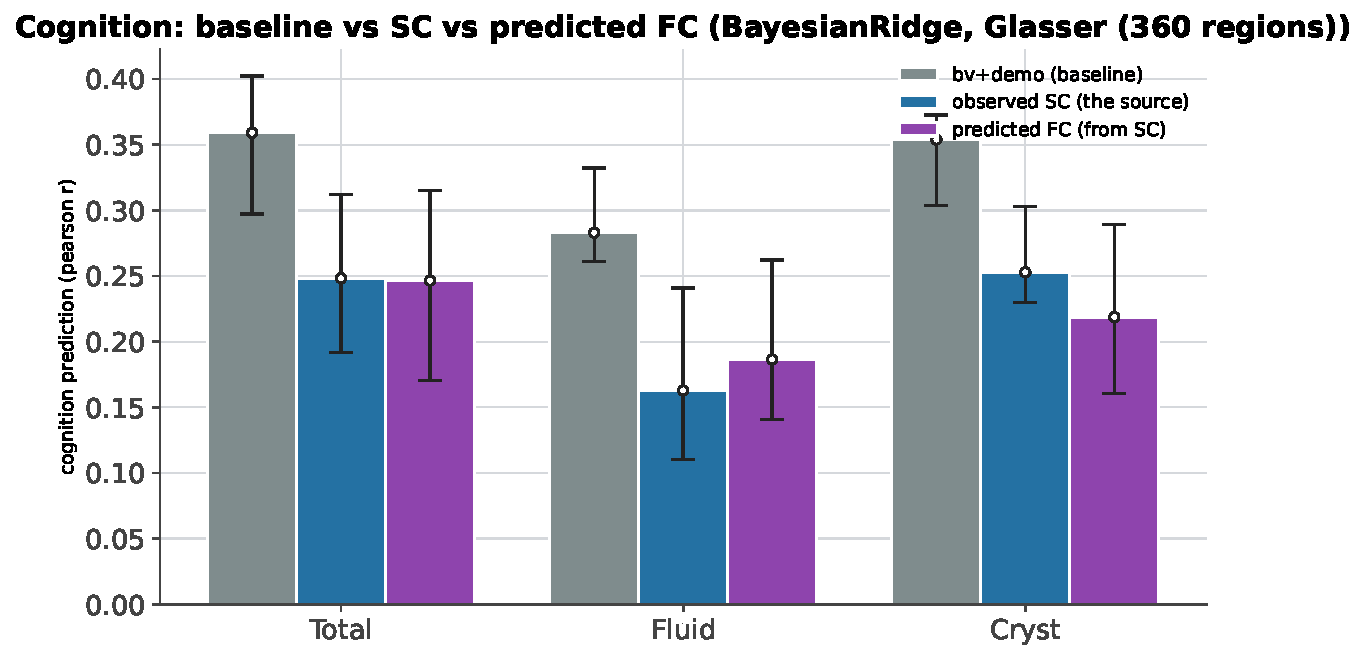
\includegraphics[height=0.66\textheight,width=\linewidth,keepaspectratio]{figures/simplified/q3_Glasser.pdf}\\[3pt]\begin{minipage}{0.95\linewidth}\scriptsize Every connectome row sits below the bv+demo baseline (grey, tallest). `Beating the source' just means less far below: predicted FC edges observed SC on CogFluid, and predicted FC+bv+demo beats observed SC+bv+demo on CogTotal and CogFluid (see table) --- a mild denoising of the weak modality. Predicted SC never beats observed FC, the strong modality.\end{minipage}\end{frame}
\section{Appendix: 4S456 (4S456 backup)}
\begin{frame}{1 · Cross-modal prediction is directional\,{\footnotesize[PCA$\rightarrow$PLS]} (4S456 backup)}\vfill\centering\large
\begin{tabular}{@{}lc@{}}\toprule \textbf{direction} & \textbf{demeaned r} \\\midrule FC$\rightarrow$SC & 0.146 \\ SC$\rightarrow$FC & 0.087 \\\midrule \textbf{ratio} & \textbf{1.68$\times$} \\\bottomrule\end{tabular}\vfill\end{frame}
\begin{frame}{1 · Cross-modal prediction is directional\,{\footnotesize[PCA$\rightarrow$PLS]} (4S456 backup)}\centering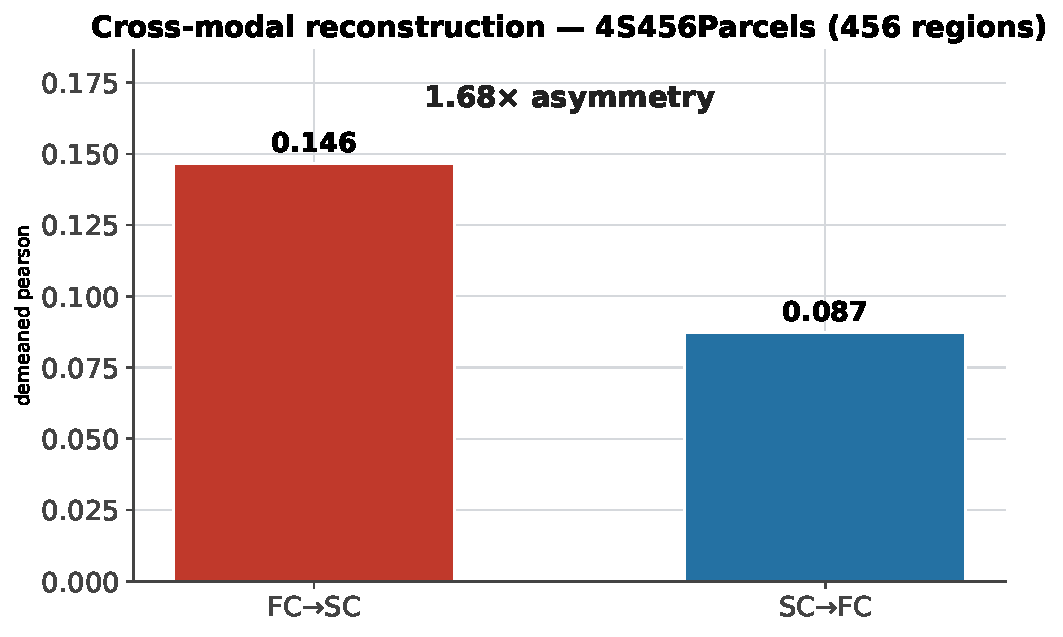
\includegraphics[height=0.66\textheight,width=\linewidth,keepaspectratio]{figures/simplified/asym_4S456Parcels.pdf}\\[3pt]\begin{minipage}{0.95\linewidth}\scriptsize Across all three models the FC$\rightarrow$SC bars are $\sim$1.6$\times$ taller than SC$\rightarrow$FC: FC reconstructs SC's individual deviations far better than the reverse, and the ratio barely changes by model, so it is not an estimator artifact. Whisker = 25th--75th percentile across the 10 seeds; white circle = mean.\end{minipage}\end{frame}
\begin{frame}{2 · A cheap baseline beats cross-modal reconstruction\,{\footnotesize[PCA$\rightarrow$PLS]} (4S456 backup)}\vfill\centering\large
\begin{tabular}{@{}lcc@{}}\toprule \textbf{source} & \textbf{$\rightarrow$ SC} & \textbf{$\rightarrow$ FC} \\\midrule cross-modal connectome & 0.146 & 0.087 \\ brain volume (bv) & 0.185 & 0.045 \\ demographics (demo) & 0.133 & 0.105 \\ bv+demo & 0.191 & 0.094 \\ \textbf{connectome + bv+demo} & \textbf{0.184} & \textbf{0.106} \\ \bottomrule\end{tabular}\vfill\end{frame}
\begin{frame}{2 · A cheap baseline beats cross-modal reconstruction\,{\footnotesize[PCA$\rightarrow$PLS]} (4S456 backup)}\centering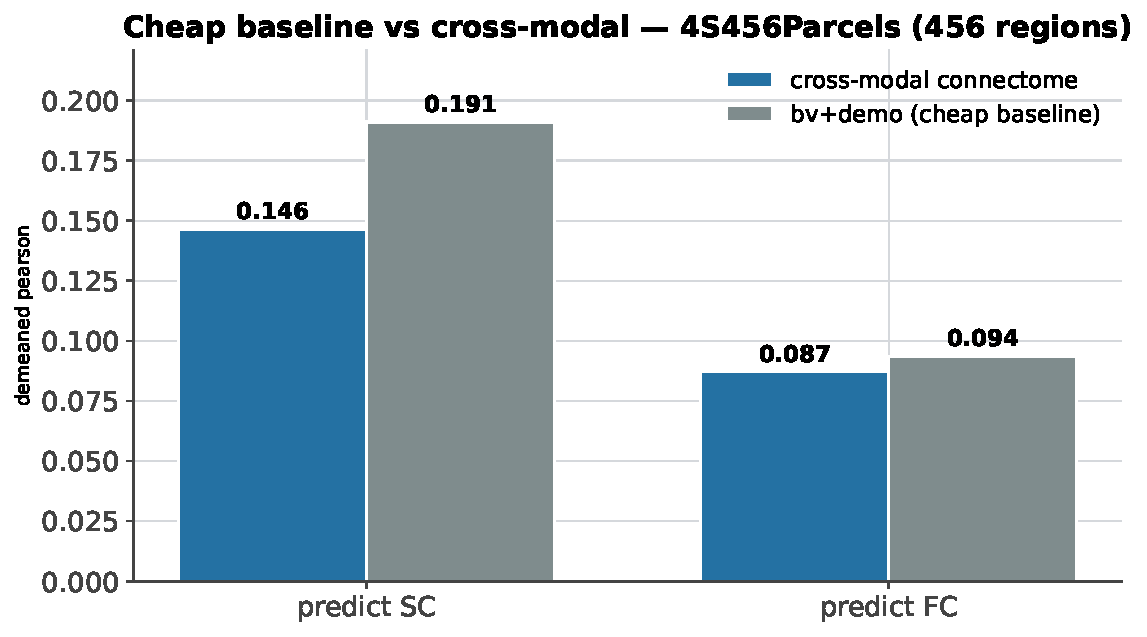
\includegraphics[height=0.66\textheight,width=\linewidth,keepaspectratio]{figures/simplified/baseline_4S456Parcels.pdf}\\[3pt]\begin{minipage}{0.95\linewidth}\scriptsize For \emph{both} targets bv+demo matches or beats the cross-modal connectome: a cheap age+sex+volume vector reconstructs the missing connectome as well as the other modality does. Adding the connectome on top of bv+demo (gold) gives only a marginal extra, so the connectome adds little beyond subject information. Note the dissociation: bv (volume) wins for SC, demo wins for FC.\end{minipage}\end{frame}
\begin{frame}{3a · Predicting SC: every metric\,{\footnotesize[PCA$\rightarrow$PLS]} (4S456 backup)}\vfill\centering\small
\begin{tabular}{@{}lcccccc@{}}\toprule \textbf{input} & \textbf{demeaned r} & \textbf{raw r} & \textbf{top1} & \textbf{avg rank} & \textbf{mse} & \textbf{r$^2$} \\\midrule FC$\rightarrow$SC & 0.146 & 0.911 & 0.151 & 0.897 & 0.004 & -0.017 \\ bv$\rightarrow$SC & 0.185 & 0.913 & 0.129 & 0.903 & 0.004 & 0.015 \\ demo$\rightarrow$SC & 0.133 & 0.912 & 0.023 & 0.764 & 0.004 & -0.001 \\ bv+demo$\rightarrow$SC & 0.191 & 0.913 & 0.173 & 0.908 & 0.004 & 0.010 \\ \textbf{FC+bv+demo$\rightarrow$SC} & \textbf{0.184} & \textbf{0.912} & \textbf{0.232} & \textbf{0.938} & \textbf{0.004} & \textbf{-0.004} \\ \bottomrule\end{tabular}\vfill\end{frame}
\begin{frame}{3a · Predicting SC: comparable metrics\,{\footnotesize[PCA$\rightarrow$PLS]} (4S456 backup)}\centering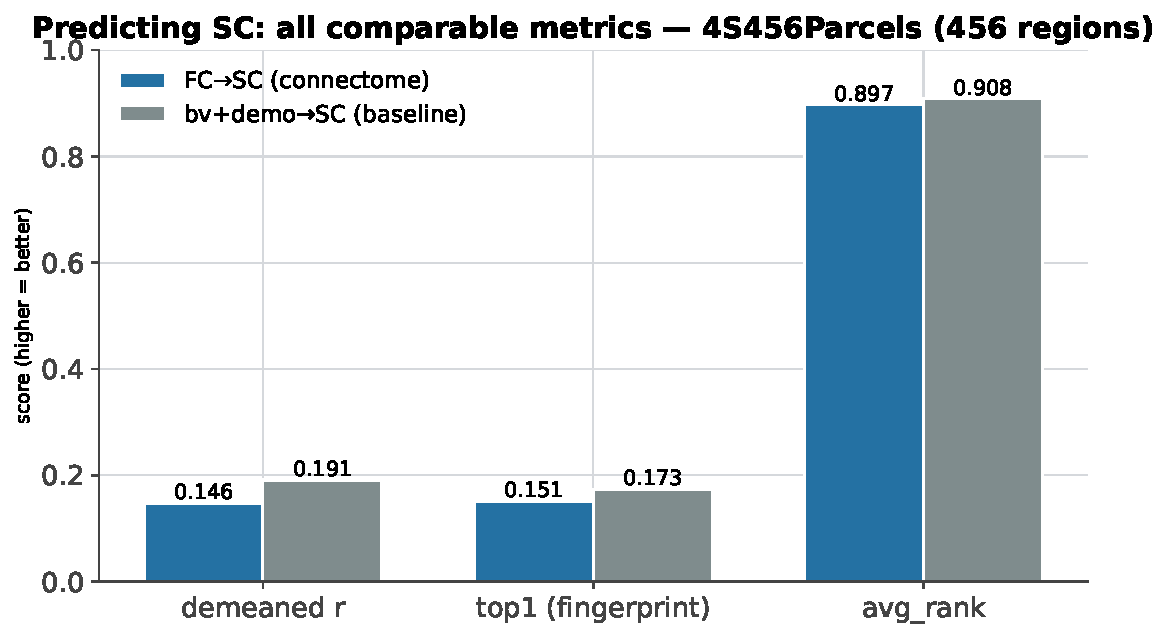
\includegraphics[height=0.66\textheight,width=\linewidth,keepaspectratio]{figures/simplified/metrics_SC_4S456Parcels.pdf}\\[3pt]\begin{minipage}{0.95\linewidth}\scriptsize Raw r is $\sim$0.9 for every input (dominated by the shared group-mean connectome, so uninformative); demeaned r is the honest individual-deviation metric, where bv+demo leads. Whisker = 25th--75th percentile over the 10 seeds.\end{minipage}\end{frame}
\begin{frame}{3b · Predicting FC: every metric\,{\footnotesize[PCA$\rightarrow$PLS]} (4S456 backup)}\vfill\centering\small
\begin{tabular}{@{}lcccccc@{}}\toprule \textbf{input} & \textbf{demeaned r} & \textbf{raw r} & \textbf{top1} & \textbf{avg rank} & \textbf{mse} & \textbf{r$^2$} \\\midrule SC$\rightarrow$FC & 0.087 & 0.813 & 0.049 & 0.730 & 0.013 & -0.047 \\ bv$\rightarrow$FC & 0.045 & 0.817 & 0.010 & 0.625 & 0.012 & -0.022 \\ demo$\rightarrow$FC & 0.105 & 0.821 & 0.013 & 0.677 & 0.012 & -0.004 \\ bv+demo$\rightarrow$FC & 0.094 & 0.818 & 0.024 & 0.687 & 0.012 & -0.020 \\ \textbf{SC+bv+demo$\rightarrow$FC} & \textbf{0.106} & \textbf{0.815} & \textbf{0.055} & \textbf{0.758} & \textbf{0.013} & \textbf{-0.040} \\ \bottomrule\end{tabular}\vfill\end{frame}
\begin{frame}{3b · Predicting FC: comparable metrics\,{\footnotesize[PCA$\rightarrow$PLS]} (4S456 backup)}\centering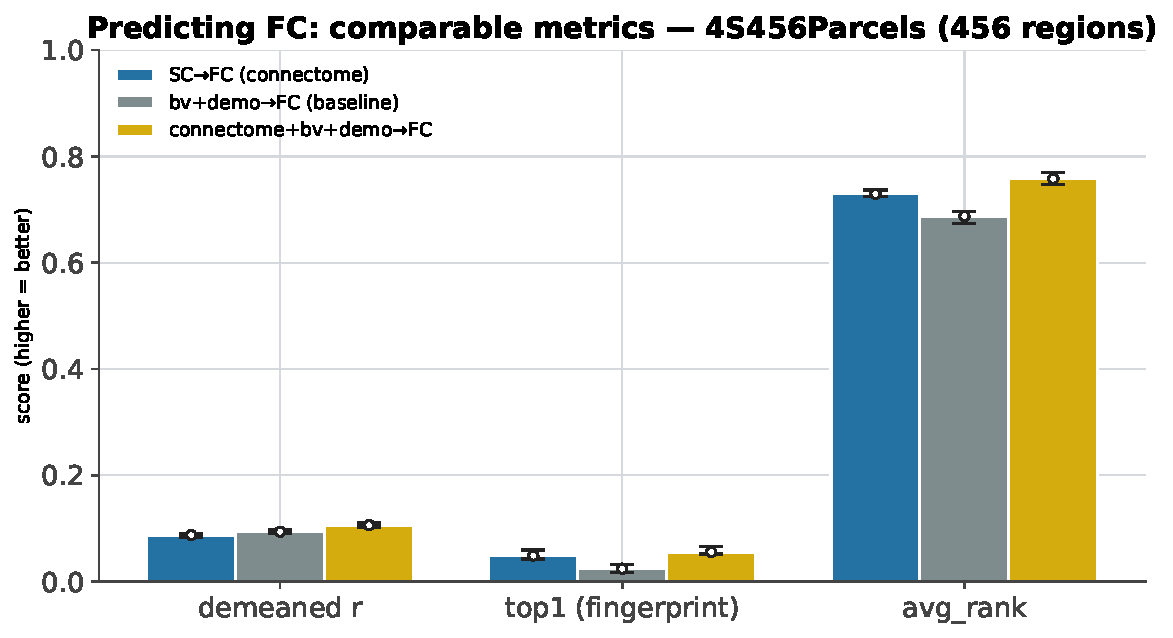
\includegraphics[height=0.66\textheight,width=\linewidth,keepaspectratio]{figures/simplified/metrics_FC_4S456Parcels.pdf}\\[3pt]\begin{minipage}{0.95\linewidth}\scriptsize Same picture predicting FC, with one twist: the real connectome (SC) beats bv+demo on the fingerprint metrics (top1, avg rank), i.e.\ it carries subject-identity information the cheap baseline lacks.\end{minipage}\end{frame}
\begin{frame}{4 · Downstream cognition: only observed FC helps\,{\footnotesize[BayesianRidge]} (4S456 backup)}\vfill\centering\footnotesize
\begin{tabular}{@{}lcccc@{}}\toprule \textbf{input} & \textbf{CogCryst r} & \textbf{Total lift} & \textbf{Fluid lift} & \textbf{Cryst lift} \\\midrule bv+demo (baseline) & 0.354 & +0.000 & +0.000 & +0.000 \\ \textbf{observed FC} & \textbf{0.476} & \textbf{+0.086} & \textbf{+0.037} & \textbf{+0.122} \\ observed SC & 0.259 & -0.103 & -0.118 & -0.095 \\ observed FC + SC & 0.475 & +0.087 & +0.043 & +0.121 \\ \textbf{observed FC + bv+demo} & \textbf{0.500} & \textbf{+0.109} & \textbf{+0.062} & \textbf{+0.146} \\ observed SC + bv+demo & 0.312 & -0.052 & -0.077 & -0.042 \\ predicted SC & 0.342 & -0.005 & -0.010 & -0.012 \\ predicted FC & 0.245 & -0.088 & -0.072 & -0.109 \\ predicted SC + bv+demo & 0.410 & +0.048 & +0.042 & +0.056 \\ predicted FC + bv+demo & 0.326 & -0.025 & -0.024 & -0.028 \\ \bottomrule\end{tabular}\vfill\end{frame}
\begin{frame}{4 · Downstream cognition: only observed FC helps\,{\footnotesize[BayesianRidge]} (4S456 backup)}\centering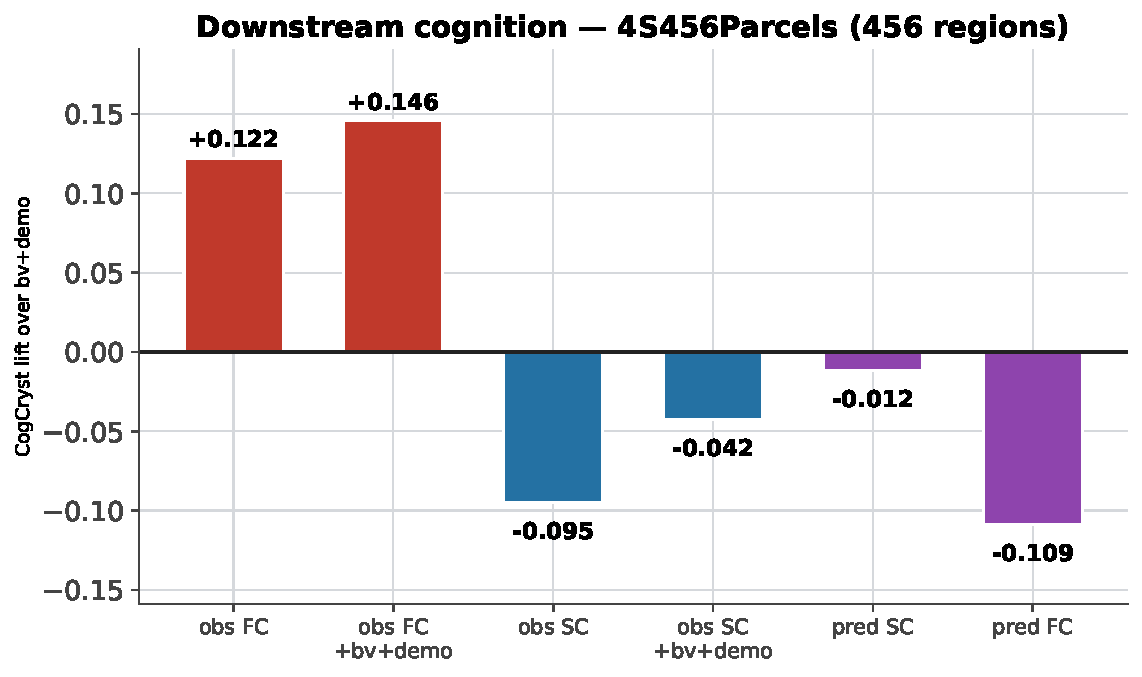
\includegraphics[height=0.66\textheight,width=\linewidth,keepaspectratio]{figures/simplified/cog_4S456Parcels.pdf}\\[3pt]\begin{minipage}{0.95\linewidth}\scriptsize Only observed FC and observed FC+bv+demo rise above zero (beat the baseline). Observed SC and both predicted connectomes sit at or below zero; predicted FC is actively harmful. Wide whiskers (25--75th pct over seeds) show even the FC lift is variable.\end{minipage}\end{frame}
\begin{frame}{5 · Downstream family: the predicted connectome carries it\,{\footnotesize[PCA$\rightarrow$PLS]} (4S456 backup)}\vfill\centering\small
\begin{tabular}{@{}lccc@{}}\toprule \textbf{predictor} & \textbf{MZ} & \textbf{DZ} & \textbf{sibling} \\\midrule observed SC & 0.999 & 0.958 & 0.884 \\ observed FC & 0.991 & 0.886 & 0.821 \\ predicted SC (raw) & 0.981 & 0.793 & 0.670 \\ \textbf{predicted SC (demog removed)} & \textbf{0.994} & \textbf{0.847} & \textbf{0.816} \\ predicted FC (raw) & 0.967 & 0.807 & 0.726 \\ predicted FC (demog removed) & 0.966 & 0.797 & 0.769 \\ \textbf{combined predicted SC} & \textbf{0.908} & \textbf{0.691} & \textbf{0.501} \\ bv+demo baseline & 0.949 & 0.791 & 0.565 \\ \bottomrule\end{tabular}\vfill\end{frame}
\begin{frame}{5 · Downstream family: the predicted connectome carries it\,{\footnotesize[PCA$\rightarrow$PLS]} (4S456 backup)}\centering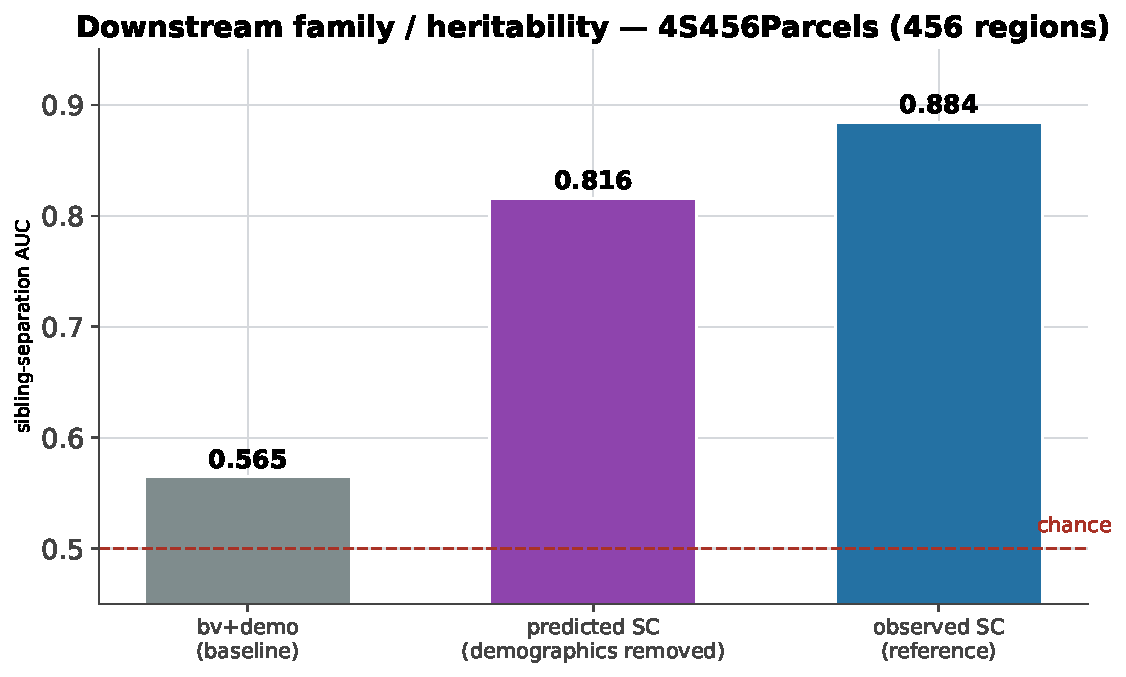
\includegraphics[height=0.66\textheight,width=\linewidth,keepaspectratio]{figures/simplified/family_4S456Parcels.pdf}\\[3pt]\begin{minipage}{0.95\linewidth}\scriptsize Predicted SC separates siblings far above the bv+demo baseline and close to observed SC: the predicted connectome keeps heritable family structure. Whisker = bootstrap 95\% CI (family is a single pipeline with no seed split).\end{minipage}\end{frame}
\begin{frame}{6 · Are the results model-dependent? (4S456 backup)}\vfill\centering\footnotesize Headlines replicate across models; the only divergences are PLS's low oracle and KernelRidge's unstable scalar rows.\\[6pt]\begin{tabular}{@{}lccc@{}}\toprule \textbf{reconstruction} & \textbf{PCA$\rightarrow$PLS} & \textbf{BayesianRidge} & \textbf{KernelRidge} \\\midrule FC$\rightarrow$SC & 0.146 & 0.171 & 0.143 \\ SC$\rightarrow$FC & 0.087 & 0.101 & 0.083 \\ \textbf{asymmetry ratio} & \textbf{1.68$\times$} & \textbf{1.70$\times$} & \textbf{1.73$\times$} \\ SC$\rightarrow$SC oracle & 0.386 & 0.622 & 0.621 \\ \bottomrule\end{tabular}\\[8pt]\begin{tabular}{@{}lccc@{}}\toprule \textbf{CogCryst lift} & \textbf{PCA$\rightarrow$PLS} & \textbf{BayesianRidge} & \textbf{KernelRidge} \\\midrule obs FC & +0.137 & +0.122 & +0.176 \\ obs SC & -0.047 & -0.095 & +0.094 \\ pred FC & -0.101 & -0.109 & -0.014 \\ \bottomrule\end{tabular}\vfill\end{frame}
\begin{frame}{6 · Are the results model-dependent? (4S456 backup)}\centering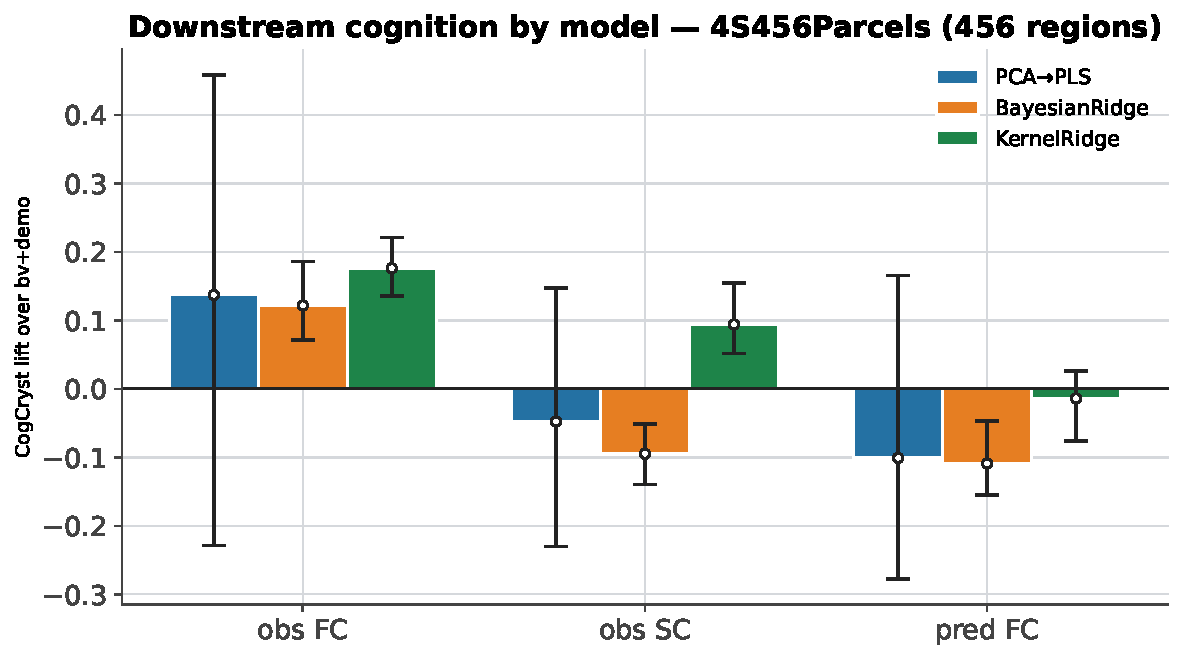
\includegraphics[height=0.66\textheight,width=\linewidth,keepaspectratio]{figures/simplified/models_4S456Parcels.pdf}\\[3pt]\begin{minipage}{0.95\linewidth}\scriptsize The observed-FC cognition lift is positive under all three models, but the negatives (obs SC, pred FC) flip sign under KernelRidge (green): KernelRidge's scalar regression is numerically unstable, which is why cognition is reported with BayesianRidge.\end{minipage}\end{frame}
\end{document}